\documentclass[]{report}

%%%% Template Packages %%%%

%\usepackage[usenames]{color}
%\usepackage{xcolor}
%\usepackage{makeidx}
%\usepackage{graphicx}
%\usepackage{epsfig}
%\usepackage{xspace}
%\usepackage{pstricks}
%\usepackage{pst-node}
%\usepackage{pst-tree}
%\usepackage{pst-plot}
%\usepackage[nonumberlist, toc, style=super]{glossaries}
\usepackage[colorlinks]{hyperref}
%\usepackage{zed-csp}
%\usepackage{psfrag}
%\usepackage{ae}
%\usepackage{txfonts}
%\usepackage{ifthen}  
%\usepackage{alltt}
%\usepackage{url} 
%\usepackage{epsfig}
%\usepackage{listings}
%\usepackage{color,listings}
%\usepackage{rotating}
%\usepackage{longtable}
%\usepackage{fancyhdr}
%\usepackage[colorinlistoftodos]{todonotes}
%\usepackage{multirow}
%\usepackage{subfig}
%\usepackage{tabularx}
%\usepackage{array}
\usepackage[utf8]{inputenc}
%\usepackage{acronym}
\usepackage{setspace}

%\usepackage{titlesec}


%\usepackage{graphicx} % Required to insert images
%\usepackage{float}
%\usepackage{listings}

\usepackage{amsmath}
\usepackage{amsthm}
\usepackage{amssymb}

\usepackage{natbib}
\usepackage[nottoc,notlot,notlof]{tocbibind}

\usepackage{tikz}
\usetikzlibrary{backgrounds}
\usetikzlibrary{arrows}

\usepackage{algorithm}
\usepackage{algpseudocode}
\usepackage{algorithmicx}

\usepackage{subcaption}
%%%%%%%%%%%%%% GENERAL %%%%%%%%%%%%%%
\newcommand{\ct}{\sim}

\newcommand{\ms}[1]{\overset{#1}{\leftarrow}}
\newcommand{\mt}[1]{\overset{#1}{\rightarrow}}

%%%%%%%%%%%%%% GG %%%%%%%%%%%%%%
\newcommand{\neigh}[1]{\operatorname{neigh}_{#1}}
\newcommand{\isomorph}{\cong}
\newcommand{\scont}[2]{\eta_{#1}(#2)}
\newcommand{\cont}[2]{\operatorname{cont}_{#1}(#2)}
\newcommand{\emb}[1]{\operatorname{emb}(#1)}
\newcommand{\allgraphs}[1]{\mathcal{G}_{#1}}
\newcommand{\startG}[1]{Z_{#1}}
\newcommand{\pro}{\to}

%%%%%%%%%%%%%% TGG %%%%%%%%%%%%%%
\newcommand{\alltgraphs}[1]{\mathcal{TG}_{#1}}
\newcommand{\startTG}[1]{Z_{#1}}
\newcommand{\emptyTG}{\varepsilon}
\newcommand{\source}{\operatorname{s}}
\newcommand{\Source}{\operatorname{S}}
\newcommand{\target}{\operatorname{t}}
\newcommand{\Target}{\operatorname{T}}
\newcommand{\cderiv}[3]{
	\ifx\relax#2\relax%
	\overset{#1}{\Rrightarrow}_{#3}%
	\else
	\overset{#1,#2}{\Rrightarrow}_{#3}%
	\fi
}
\newcommand{\deriv}[3]{
	\ifx\relax#2\relax
	\overset{#1}{\Rightarrow}_{#3}
	\else
	\overset{#1,#2}{\Rightarrow}_{#3}
	\fi
}
\newcommand{\derivtr}[1]{
	\Rightarrow^*_{#1}
}
\newcommand{\tcderiv}[3]{
	\ifx\relax#2\relax
	\overset{#1}{\Rrightarrow}_{#3}
	\else
	\overset{#1,#2}{\Rrightarrow}_{#3}
	\fi
}
\newcommand{\tderiv}[3]{
	\ifx\relax#2\relax
	\overset{#1}{\Rightarrow}_{#3}
	\else
	\overset{#1,#2}{\Rightarrow}_{#3}
	\fi
}
\newcommand{\tderivtr}[1]{\Rightarrow^*_{#1}}

%%%% PAC %%%%
\newcommand{\cderivpac}[4]{\overset{#1,#2,#3}{\Rrightarrow}_{#4}}
\newcommand{\derivpac}[4]{
	\ifx\relax#3\relax
	\overset{#1,#2}{\Rightarrow}_{#4}
	\else
	\overset{#1,#2,#3}{\Rightarrow}_{#4}
	\fi}
\newcommand{\derivpacn}[2]{\Rightarrow^{#2}_{#1}}
\newcommand{\resolv}[1]{\overset{#1}{\rightarrowtail}}
\newcommand{\resolvn}[2]{\overset{#1}{\rightarrowtail}^{#2}}
\newcommand{\derivpactr}[1]{\Rightarrow^*_{#1}}
\newcommand{\resolvtr}[1]{\rightarrowtail^*}

\newcommand{\tcderivpac}[4]{\overset{#1,#2,#3}{\Rrightarrow}_{#4}}
\newcommand{\tderivpac}[4]{
	\ifx\relax#3\relax
	\overset{#1,#2}{\Rightarrow}_{#4}
	\else
	\overset{#1,#2,#3}{\Rightarrow}_{#4}
	\fi
}
\newcommand{\tderivpacn}[2]{\Rightarrow^{#2}_{#1}}
\newcommand{\tresolv}[1]{\overset{#1}{\rightarrowtail}}
\newcommand{\tresolvn}[2]{\overset{#1}{\rightarrowtail}^{#2}}
\newcommand{\tderivpactr}[1]{\Rightarrow^*_{#1}}
\newcommand{\tresolvtr}[1]{\rightarrowtail^*_{#1}}



%%%%%%%%%%%%%% TIKZ %%%%%%%%%%%%%%
\tikzstyle{grammar}=[shorten >= 1pt, ->, draw=black!50, framed, background rectangle/.style={draw, rounded corners}, font=\scriptsize ]
\tikzstyle{graph}=[shorten >= 1pt, ->, draw=black!50, font=\scriptsize]
\tikzstyle{rid} = [inner sep=3pt, align=left, anchor=east]
\tikzstyle{nont}=[rectangle, inner sep=3pt, draw, fill=white, minimum width=5pt]
\tikzstyle{t}=[circle, inner sep=1pt, draw, fill=white, minimum width=5pt]
\tikzstyle{pac}=[circle, inner sep=1pt, draw, dotted, fill=white, minimum width=5pt]
\tikzstyle{empty}=[font=\Large, fill=white]
\tikzstyle{g}=[inner sep=3pt, fill=white]
\tikzstyle{lhs}=[inner sep=1pt, fill=white]
\tikzstyle{w}=[circle, inner sep=1pt, below=8pt, draw, fill=white, font=\tiny]
\tikzstyle{uw}=[circle, inner sep=1pt, above=8pt, draw, fill=white, font=\tiny]
\tikzstyle{edge}=[->, thin, -latex]
\tikzstyle{pacedge}=[->, thin, -latex, dotted]
\tikzstyle{edgeLabel}=[midway, above]
\tikzstyle{vledgeLabel}=[midway, left]
\tikzstyle{vredgeLabel}=[midway, right]
\tikzstyle{vbedgeLabel}=[above=3pt]
\tikzstyle{wedge}=[-, thin]
\tikzstyle{biedge}=[-, thin]
\tikzstyle{pipe}=[-, thick]
\tikzstyle{morph}=[-, thin, dashed, -latex]

\newcommand{\ridX}{-0.3}
\newcommand{\ridY}{0.5}
\newcommand{\lhsX}{-0.3}
\newcommand{\pipeUY}{-0.5}
\newcommand{\pipeBY}{0.5}

%% Scheme %%
\tikzstyle{scheme}=[shorten >= 1pt, ->, draw=black!50, framed, background rectangle/.style={draw, rounded corners}, font=\scriptsize ]
\tikzstyle{object}=[rectangle, inner sep=3pt, draw, fill=white, minimum width=5pt]
\tikzstyle{metaobject}=[rectangle, inner sep=3pt, draw, dashed, fill=white, minimum width=5pt]
\tikzstyle{activity}=[rectangle, inner sep=3pt, draw, fill=white, minimum width=5pt, rounded corners]

% Title Page
\title{}
\author{William Bombardelli da Silva}


\begin{document}
\maketitle

\begin{abstract}
\end{abstract}

\section{Theoretical Review}
In this section, we introduce the theoretical concepts used along this thesis. The definitions below are taken from the works of ...%TODO: cite 27, 54,s_99.
We first go on to define graphs and graph grammars and then, building upon it, we construct the so-called triple graph grammars.

\subsection{Graph Grammars}
We start presenting our notation for graphs and grammars, accompanied by examples, then we introduce the dynamic aspects of the graph grammar formalism that is, how graph grammars are to be interpreted.

%%%%%% Abstract Syntax %%%%%%

%TODO: Maybe change this definition layout
\begin{definition}
	\label{def:graph}
	A directed labeled graph $G$ over the set of symbols $\Sigma$, $G = (V, E, \phi)$ consists of a finite set of vertices $V$, a set of labeled directed edges $E \subseteq V \times \Sigma \times V$ and a total vertex labeling function $\phi : V \to \Sigma$. Directed labeled graphs are often referred to simply as graphs. For a fixed graph $G$ we refer to its components as $V_G$, $E_G$ and $\phi_G$. Moreover, we define the special empty graph as $\emptyGraph := (\emptyset, \emptyset, \emptyset)$ and we denote the set of all graphs over $\Sigma$ by $\allgraphs{\Sigma}$.
	%TODO: Talk about muti-edges, loops, etc?
	%TODO: Comments about notation (e..g edge labels x vertex labels)
	
	If $\phi_G(v) = a$ we say $v$ is labeled by $a$. Two vertices $v$ and $w$ are neighbors (also adjacent) iff there is one or more edges between them, that is, $(v,\_,w) \in E_G \lor (w,\_,v) \in E_G$. Two graphs $G$ and $H$ are disjoint iff $V_G \cap V_H = \emptyset$.
	
	We define also de function $\neigh{G}: 2^{V_G} \to 2^{V_G}$, that applied to $U$ gives the set of neighbors of vertices in $U$ minus $U$. That is $\neigh{G}(U) = \{ v \in V_G \setminus U \st \text{ exists a } (v,l,u) \in E_G \text{ or a } (u,l,v) \in E_G \text{ with } u \in U \}$
\end{definition}

\begin{definition}
	\label{def:morphism}
	A morphism of graphs $G$ and $H$ is a total mapping $m: V_G \to V_H$.
\end{definition}

\begin{definition}
	An isomorphism of directed labeled graphs $G$ and $H$ is a bijective mapping $m: V_G \to V_H$ that maintains the connections between vertices and their labels, that is, $(v,l,w) \in E_G$ if, and only if,  $(m(v),l,m(w)) \in E_H$ and if $m(v) = w$ then $\phi_G(v) = \phi_H(w)$. In this case, $G$ and $H$ are said to be isomorphic, we write $G \isomorph H$, and we denote the equivalence class of all graphs isomorphic to G by $[G]$.
	Notice that, contrary to isomorphisms, morphism do not require bijectivity nor label or edge-preserving properties.
	%TODO: Maybe say some words about the difference to the common isomorphism
\end{definition}

\begin{definition}
	A $\Gamma\text{-boundary}$ graph $G$ is such that vertices labeled with any symbol from $\Gamma$ are not neighbors. That is, the graph $G$ is $\Gamma\text{-boundary}$ iff, $\not\exists (v,\_,w) \in E_G \. \phi_G(v) \in \Gamma \land \phi_G(w) \in \Gamma$.
\end{definition}

%TODO: comments on graphs: good for modelling

\begin{definition}
	\label{def:gg}
	An graph grammar with neighborhood-controlled embedding (NCE graph grammar) $GG = (\Sigma, \Delta \subseteq \Sigma, S \in \Sigma, P)$ consists of a finite set of symbols $\Sigma$ that is the alphabet, a subset of the alphabet $\Delta \subseteq \Sigma$ that holds the terminal symbols (we define the complementary set of non-terminal symbols as $\Gamma := \Sigma \setminus \Delta$), a special symbol of the alphabet $S \in \Sigma$ that is the start symbol, and a finite set of production rules $P$ of the form $(A \pro R, \omega)$ where $A \in \Gamma$ is the so-called left-hand side, $R \in \allgraphs{\Sigma}$ is the right-hand side and $\omega : V_R \pto 2^{\Sigma \times \Sigma}$ is the partial embedding function from the $R$'s vertices to pairs of edge and label symbols. NCE graph grammars are often referred to as graph grammars or simply as grammars.
	
	For convenience, define the start graph of $GG$ as $\startG{GG} := (\{v_s\},\emptyset,\{v_s \mapsto S\})$
	%TODO: notation for the componenents? set of all grammars?
	%TODO: Comment notation: e.g. do not separate edge vertex labels
	%TODO: also say something about more general grammars (e.g. context-free)
	%TODO: Extend here with look-ahead
	%TODO: discuss empty productions
	
	Vertices from the right-hand sides of rules labeled by non-terminal (terminal) symbols are said to be non-terminal (terminal) vertices.
\end{definition}

\begin{definition}
	A boundary graph grammar with neighborhood-controlled embedding (BNCE graph grammar) $GG$ is such that non-terminal vertices of the right-hand sides of rules are not neighbors. That is, the graph grammar $GG$ is boundary iff all its rules' right-hand sides are $\Gamma\text{-boundary}$ graphs.
\end{definition}

%TODO: comments on grammars: why? intuition...
%TODO: comment about hyperedge replacement grammars

%%%%%% Concrete Syntax %%%%%%
In the following, we present our concrete syntax inspired by the well-known backus-naur form to denote BNCE graph grammar rules. Let $GG = (\{A,a,b,c\},$ $\{a,b,c\}, A, \{p,q\})$ be a graph grammar with production rules $p = (A \pro G,\omega)$ and $q = (A \pro H,\zeta)$ where $G = (\{v_1, v_2, v_3\}, \{(v_1,l,v_2), (v_2,m,v_3)\}, \{v_1 \mapsto B, v_2 \mapsto b, v_3 \mapsto c \})$, $\omega = \{v_1 \mapsto \{(l,a), (l,b), (m,c)\}\}$, and $H = (\{u_1\}, \emptyset, \{u_1 \mapsto a\})$ and $\zeta = \emptyset$, we denote $p$ and $q$ together as\\

\noindent
\begin{equation*}
	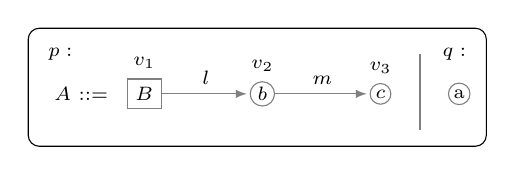
\begin{tikzpicture}[grammar]
	\node[rid] at (\ridX,\ridY) {$p:$};
	%The LHS
	\draw (\lhsX,0) node[lhs] (lhs) {$A$ ::=};
	
	%The RHS graph
	\draw (0.5,0) node[nont, label=90:$v_1$] (v1) {$B$};
	\draw (2,0) node[t, label=90:$v_2$] (v2) {$b$};
	\draw (3.5,0) node[t, label=90:$v_3$] (v3) {$c$};
	
	\draw[edge] (v1) -- (v2) node [edgeLabel] {$l$};
	\draw[edge] (v2) -- (v3) node [edgeLabel] {$m$};
	
	%The embedding
	%\draw node[w, label=0:$l;l;m$, label=-45:$a;b;c$] at (v1.south) (w-v1) {}
	%[wedge] (v1) -- (w-v1);
	
	%The next rule separator
	\draw[pipe] (4,\pipeBY) -- (4,\pipeUY);
	
	%The second RHS graph
	\node[rid] at (4.7,\ridY) {$q:$};
	\draw (4.5,0) node[t] (u1) {a};
	\end{tikzpicture}
\end{equation*}

Notice that, we use squares for non-terminal vertices, circles for terminal vertices, position the respective label inside the shape and the (possibly omitted) identifier over it. Over each edge is positioned its respective label. To depict the embedding function, we place below the respective vertex a small circle labeled with the image pairs of the embedding function for this node aligned vertically and separated by semi-colons.

%TODO: comment on the different notation compared to the literature that uses attributed graphs and squares, etc...

%%%%%% Semantics %%%%%%
With these syntactic notions of the formalism presented, we introduce below its semantics by means of the concepts of derivation step, derivation and language.

\begin{definition}
	Let $GG = (\Sigma, \Delta, S, P)$ be a graph grammar and $G$ and $H$ be two graphs over $\Sigma$ disjoint from any right-hand side from $P$, $G$ concretely derives in one step into $H$ with rule $r$ and vertex $v$, we write $G \cderiv{r}{v}{GG} H$ and call it a concrete derivation step, if, and only if, the following holds:
	\begin{align*}
		r & = (A \pro R, \omega) \in P \text{ and } A = \phi_G(v) \text{ and} \\
		V_H  & = (V_G \setminus \{v\}) \cup V_R \text{ and} \\
		E_H & = (E_G \setminus \{(w,l,t) \in E_G \st v = w \lor v = t\}) \\
		& \cup E_R \\
		& \cup \{(w,l,t) \st (w,l,v) \in E_G \land (l,\phi_G(w)) \in \omega(t)\} \\
		& \cup \{(t,l,w) \st (v,l,w) \in E_G \land (l,\phi_G(w)) \in \omega(t)\} \text{ and} \\
		\phi_H & = (\phi_G \setminus \{(v,x) \st x \in V_G \}) \cup \phi_R
	\end{align*}
	Notice that, without loss of generalization, we set $\omega(t) = \emptyset$ for all vertices $t$ without an image defined in $\omega$.
	
	If $G$ concretely derives in one step into any graph $H'$ isomorphic to $H$, we say it derives in one step into $H'$ and write $G \deriv{r}{v}{GG} H'$. 
	
	When $GG$, $r$ or $v$ are clear in the context or irrelevant we might omit them and simply write $G \cderiv{}{}{} H$ or $G \deriv{}{}{} H$. Moreover, we denote the reflexive transitive closure of $\deriv{}{}{}$ by $\derivtr{}{}{}$ and, for $G \derivtr{}{}{} H'$, we say $G$ derives in one or more steps into $H'$, or simply $G$ derives into $H'$.
\end{definition}

%TODO: give intuition for the rule application
%TODO: Notice direction does not matter in embedding. why we chose so?

\begin{definition}
	A derivation $D$ in $GG$ is a sequence of derivation steps and is written as
	\[ 
		D = (G_0 \deriv{r_0}{v_0}{} G_1 \deriv{r_1}{v_1}{} G_2 \deriv{r_2}{v_2}{} \dots \deriv{r_{n-1}}{v_{n-1}}{} G_n)
	\]
\end{definition}

\begin{definition}
	The language $L(GG)$ generated by the grammar $GG$ is the set of all graphs containing only terminal vertices derived from the start graph $\startG{GG}$, that is
	\[
		L(GG) = \{H \st \phi_H(V_H) \subseteq \Delta \land \startG{GG} \derivtr{}{}{} H\}
	\]
\end{definition}

%TODO: Notice that the labels of the edges are ignored if theu are terminal or not

Notice that for every graph $G \in L(GG)$, there is at least one finite derivation $(\startG{GG} \deriv{r_0}{v_0}{} \dots \deriv{r_{n-1}}{v_{n-1}}{} G)$, but it is not guaranteed that this derivation be unique. In the case that there are more than one derivation for a $G$, we say that the grammar $GG$ is ambiguous. 

Below we give one example of a grammar whose language consists of all chains of one or more vertices with interleaved vertices labeled with $a$ and $b$.

%Examples (chains and activities)
\begin{example}{Chains of a's and b's.}
	$GG = (\{S,A,B,a,b,c\}, \{a,b,c\}, S, P)$, where $P$ is
	
	\noindent
	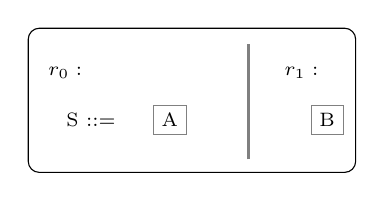
\begin{tikzpicture}[grammar]
	\node[rid] at (0,0.6) {$r_0:$};
	%The LHS
	\draw (0,0) node[lhs] (lhs) {S ::=};
	
	%The RHS graph
	\draw (1,0) node[nont] (v1) {A};
	
	%The next rule separator
	\draw[pipe] (2,-0.5) -- (2,1);
	
	%The second RHS graph
	\node[rid] at (3,0.6) {$r_1:$};
	\draw (3,0) node[nont] (v2) {B};
	\end{tikzpicture}
	
	\noindent
	\begin{minipage}[t]{.5\textwidth}
		\begin{tikzpicture}[grammar]
		\node[rid] at (0,0.6) {$r_2:$};
		%The LHS
		\draw (0,0) node[lhs] (lhs) {A ::=};
		
		%The RHS graph
		\draw (1,0) node[t] (v3) {a};
		\draw (2.5,0) node[nont] (v4) {B};
		
		\draw[edge] (v3) -- (v4) node [edgeLabel] {$c$};
		
		\draw node[w, label=0:$c$, label=-45:$b$] at (v3.south) (w-v3) {}
		[wedge] (v1) -- (w-v3);
		
		%The next rule separator
		\draw[pipe] (3.5,-1) -- (3.5,1);
		
		%The second RHS graph
		\node[rid] at (4.5,0.6) {$r_3:$};
		\draw (4.5,0) node[t] (v5) {a};
		\draw node[w, label=0:$c$, label=-45:$b$] at (v5.south) (w-v5) {}
		[wedge] (v5) -- (w-v5);
		\end{tikzpicture}
	\end{minipage}%
	\begin{minipage}[t]{.5\textwidth}
		\begin{tikzpicture}[grammar]
		\node[rid] at (0,0.6) {$r_4:$};
		%The LHS
		\draw (0,0) node[lhs] (lhs) {B ::=};
		
		%The RHS graph
		\draw (1,0) node[t] (v6) {b};
		\draw (2.5,0) node[nont] (v7) {A};
		
		\draw[edge] (v3) -- (v4) node [edgeLabel] {$c$};
		
		\draw node[w, label=0:$c$, label=-45:$a$] at (v6.south) (w-v6) {}
		[wedge] (v1) -- (w-v6);
		
		%The next rule separator
		\draw[pipe] (3.5,-1) -- (3.5,1);
		
		%The second RHS graph
		\node[rid] at (4.5,0.6) {$r_5:$};
		\draw (4.5,0) node[t] (v8) {b};
		\draw node[w, label=0:$c$, label=-45:$a$] at (v8.south) (w-v8) {}
		[wedge] (v8) -- (w-v8);
		\end{tikzpicture}
	\end{minipage}
\end{example}

The graph $G=$
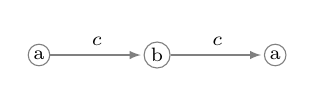
\begin{tikzpicture}[graph]
\draw (0,0) node[t] (v1) {a};
\draw (1.5,0) node[t] (v2) {b};
\draw (3,0) node[t] (v3) {a};
\draw[edge] (v1) -- (v2) node [edgeLabel] {$c$};
\draw[edge] (v2) -- (v3) node [edgeLabel] {$c$};
\end{tikzpicture}
belongs to $L(GG)$ because it contains only terminal vertices and $\startG{GG}$ derives into it using the following derivation:
\[
	\startG{GG} \deriv{r_0}{v_0}{} 
		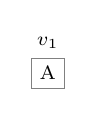
\begin{tikzpicture}[graph]
			\draw (0,0) node[nont, label=90:$v_1$] (v1) {A};
		\end{tikzpicture}
		\deriv{r_2}{v_1}{} 
		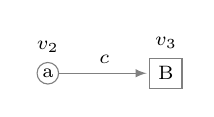
\begin{tikzpicture}[graph]
			\draw (1,0) node[t, label=90:$v_2$] (v2) {a};
			\draw (2.5,0) node[nont, label=90:$v_3$] (v3) {B};
			\draw[edge] (v2) -- (v3) node [edgeLabel] {$c$};
		\end{tikzpicture}
		\deriv{r_4}{v_3}{}
		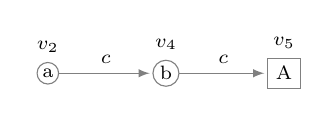
\begin{tikzpicture}[graph]
			\draw (1,0) node[t, label=90:$v_2$] (v2) {a};
			\draw (2.5,0) node[t, label=90:$v_4$] (v4) {b};
			\draw (4,0) node[nont, label=90:$v_5$] (v5) {A};
			\draw[edge] (v2) -- (v4) node [edgeLabel] {$c$};
			\draw[edge] (v4) -- (v5) node [edgeLabel] {$c$};
		\end{tikzpicture}
\]\[
		\deriv{r_3}{v_5}{}
		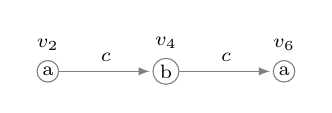
\begin{tikzpicture}[graph]
			\draw (0,0) node[t, label=90:$v_2$] (v2) {a};
			\draw (1.5,0) node[t, label=90:$v_4$] (v4) {b};
			\draw (3,0) node[t, label=90:$v_6$] (v6) {a};
			\draw[edge] (v2) -- (v4) node [edgeLabel] {$c$};
			\draw[edge] (v4) -- (v6) node [edgeLabel] {$c$};
		\end{tikzpicture}
\]

%TODO: Adapt activty diagram afterwards
%\begin{example}{Activity diagrams.}
	$GG = (\{S,A,F,D,L,a,c,e,if\}, \{a,c,e,if\}, P, S)$, where $P$ is\\
	
	\noindent
	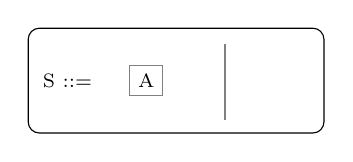
\begin{tikzpicture}[grammar]
	%The LHS
	\draw (0,0) node[lhs] (lhs) {S ::=};
	
	%The RHS graph
	\draw (1,0) node[nont] (v1) {A};
	
	%The next rule separator
	\draw[pipe] (2,-0.5) -- (2,0.5);
	
	%The second RHS graph
	\draw (3,0) node[g] (v2) {$\emptyGraph$};
	\end{tikzpicture}
	
	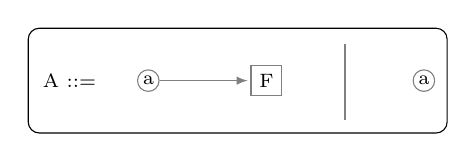
\begin{tikzpicture}[grammar]
	%The LHS
	\draw (0,0) node[lhs] (lhs) {A ::=};
	
	%The RHS graph
	\draw (1,0) node[t] (v1) {a};
	\draw (2.5,0) node[nont] (v2) {F};
	
	\draw[edge] (v1) -- (v2);
	
	%The next rule separator
	\draw[pipe] (3.5,-0.5) -- (3.5,0.5);
	
	%The second RHS graph
	\draw (4.5,0) node[t] (v3) {a};
	\end{tikzpicture}
	
	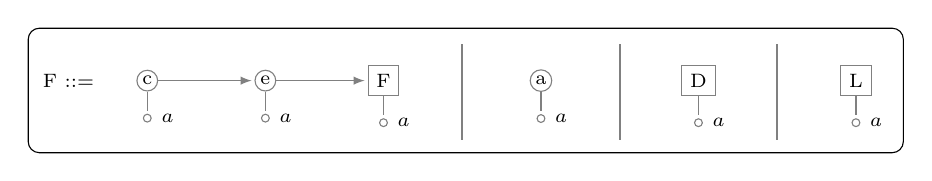
\begin{tikzpicture}[grammar]
	%The LHS
	\draw (0,0) node[lhs] (lhs) {F ::=};
	
	%The RHS graph
	\draw (1,0) node[t] (v1) {c};
	\draw (2.5,0) node[t] (v2) {e};
	\draw (4,0) node[nont] (v3) {F};
	
	\draw[edge] (v1) -- (v2);
	\draw[edge] (v2) -- (v3);
	
	\draw node[w, label=0:$a$] at (v1.south) (w-v1) {}
	[wedge] (v1) -- (w-v1);
	\draw node[w, label=0:$a$] at (v2.south) (w-v2) {}
	[wedge] (v2) -- (w-v2);
	\draw node[w, label=0:$a$] at (v3.south) (w-v3) {}
	[wedge] (v3) -- (w-v3);
	
	%The next rule separator
	\draw[pipe] (5,-0.75) -- (5,0.5);
	
	%The second RHS graph
	\draw (6,0) node[t] (v4) {a};
	\draw node[w, label=0:$a$] at (v4.south) (w-v4) {}
	[wedge] (v4) -- (w-v4);
	
	%The next rule separator
	\draw[pipe] (7,-0.75) -- (7,0.5);
	
	%The second RHS graph
	\draw (8,0) node[nont] (v5) {D};
	\draw node[w, label=0:$a$] at (v5.south) (w-v5) {}
	[wedge] (v5) -- (w-v5);
	
	%The next rule separator
	\draw[pipe] (9,-0.75) -- (9,0.5);
	
	%The second RHS graph
	\draw (10,0) node[nont] (v6) {L};
	\draw node[w, label=0:$a$] at (v6.south) (w-v6) {}
	[wedge] (v6) -- (w-v6);
	\end{tikzpicture}
	
	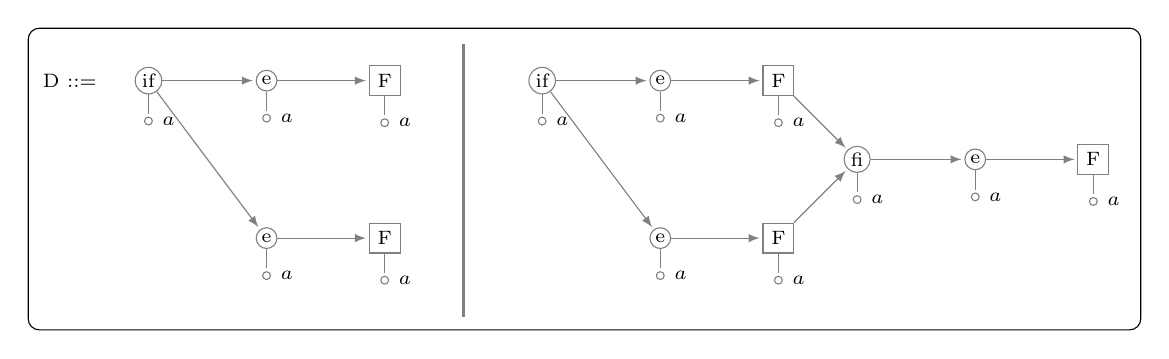
\begin{tikzpicture}[grammar]
	%The LHS
	\draw (0,0) node[lhs] (lhs) {D ::=};
	
	%The RHS graph
	\draw (1,0) node[t] (v1) {if};
	\draw (2.5,0) node[t] (v2) {e};
	\draw (4,0) node[nont] (v3) {F};
	\draw (2.5,-2) node[t] (v4) {e};
	\draw (4,-2) node[nont] (v5) {F};
	
	\draw[edge] (v1) -- (v2);
	\draw[edge] (v2) -- (v3);
	\draw[edge] (v1) -- (v4);
	\draw[edge] (v4) -- (v5);
	
	\draw node[w, label=0:$a$] at (v1.south) (w-v1) {}
	[wedge] (v1) -- (w-v1);
	\draw node[w, label=0:$a$] at (v2.south) (w-v2) {}
	[wedge] (v2) -- (w-v2);
	\draw node[w, label=0:$a$] at (v3.south) (w-v3) {}
	[wedge] (v3) -- (w-v3);
	\draw node[w, label=0:$a$] at (v4.south) (w-v4) {}
	[wedge] (v4) -- (w-v4);
	\draw node[w, label=0:$a$] at (v5.south) (w-v5) {}
	[wedge] (v5) -- (w-v5);
	
	%The next rule separator
	\draw[pipe] (5,-3) -- (5,0.5);
	
	%The second RHS graph
	\draw (6,0) node[t] (v6) {if};
	\draw (7.5,0) node[t] (v7) {e};
	\draw (9,0) node[nont] (v8) {F};
	\draw (7.5,-2) node[t] (v9) {e};
	\draw (9,-2) node[nont] (v10) {F};
	\draw (10,-1) node[t] (v11) {fi};
	\draw (11.5,-1) node[t] (v12) {e};
	\draw (13,-1) node[nont] (v13) {F};
	
	
	\draw[edge] (v6) -- (v7);
	\draw[edge] (v7) -- (v8);
	\draw[edge] (v6) -- (v9);
	\draw[edge] (v9) -- (v10);
	\draw[edge] (v10) -- (v11);
	\draw[edge] (v8) -- (v11);
	\draw[edge] (v11) -- (v12);
	\draw[edge] (v12) -- (v13);
	
	\draw node[w, label=0:$a$] at (v6.south) (w-v6) {}
	[wedge] (v6) -- (w-v6);
	\draw node[w, label=0:$a$] at (v7.south) (w-v7) {}
	[wedge] (v7) -- (w-v7);
	\draw node[w, label=0:$a$] at (v8.south) (w-v8) {}
	[wedge] (v8) -- (w-v8);
	\draw node[w, label=0:$a$] at (v9.south) (w-v9) {}
	[wedge] (v9) -- (w-v9);
	\draw node[w, label=0:$a$] at (v10.south) (w-v10) {}
	[wedge] (v10) -- (w-v10);
	\draw node[w, label=0:$a$] at (v11.south) (w-v11) {}
	[wedge] (v11) -- (w-v11);
	\draw node[w, label=0:$a$] at (v12.south) (w-v12) {}
	[wedge] (v12) -- (w-v12);
	\draw node[w, label=0:$a$] at (v13.south) (w-v13) {}
	[wedge] (v13) -- (w-v13);
	\end{tikzpicture}
	
	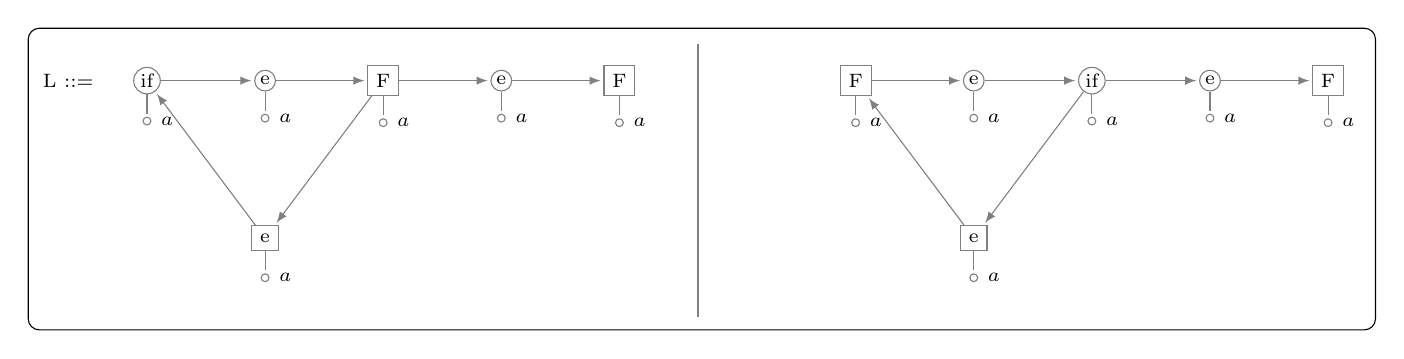
\begin{tikzpicture}[grammar]
	%The LHS
	\draw (0,0) node[lhs] (lhs) {L ::=};
	
	%The RHS graph
	\draw (1,0) node[t] (v1) {if};
	\draw (2.5,0) node[t] (v2) {e};
	\draw (4,0) node[nont] (v3) {F};
	\draw (5.5,0) node[t] (v4) {e};
	\draw (7,0) node[nont] (v5) {F};
	\draw (2.5,-2) node[nont] (v6) {e};
	
	\draw[edge] (v1) -- (v2);
	\draw[edge] (v2) -- (v3);
	\draw[edge] (v3) -- (v4);
	\draw[edge] (v4) -- (v5);
	\draw[edge] (v3) -- (v6);
	\draw[edge] (v6) -- (v1);
	
	\draw node[w, label=0:$a$] at (v1.south) (w-v1) {}
	[wedge] (v1) -- (w-v1);
	\draw node[w, label=0:$a$] at (v2.south) (w-v2) {}
	[wedge] (v2) -- (w-v2);
	\draw node[w, label=0:$a$] at (v3.south) (w-v3) {}
	[wedge] (v3) -- (w-v3);
	\draw node[w, label=0:$a$] at (v4.south) (w-v4) {}
	[wedge] (v4) -- (w-v4);
	\draw node[w, label=0:$a$] at (v5.south) (w-v5) {}
	[wedge] (v5) -- (w-v5);
	\draw node[w, label=0:$a$] at (v6.south) (w-v6) {}
	[wedge] (v6) -- (w-v6);
	
	%The next rule separator
	\draw[pipe] (8,-3) -- (8,0.5);
	
	%The second RHS graph
	\draw (10,0) node[nont] (v7) {F};
	\draw (11.5,0) node[t] (v8) {e};
	\draw (13,0) node[t] (v9) {if};
	\draw (14.5,0) node[t] (v10) {e};
	\draw (16,0) node[nont] (v11) {F};
	\draw (11.5,-2) node[nont] (v12) {e};
	
	\draw[edge] (v7) -- (v8);
	\draw[edge] (v8) -- (v9);
	\draw[edge] (v9) -- (v10);
	\draw[edge] (v10) -- (v11);
	\draw[edge] (v9) -- (v12);
	\draw[edge] (v12) -- (v7);
	
	\draw node[w, label=0:$a$] at (v7.south) (w-v7) {}
	[wedge] (v7) -- (w-v7);
	\draw node[w, label=0:$a$] at (v8.south) (w-v8) {}
	[wedge] (v8) -- (w-v8);
	\draw node[w, label=0:$a$] at (v9.south) (w-v9) {}
	[wedge] (v9) -- (w-v9);
	\draw node[w, label=0:$a$] at (v10.south) (w-v10) {}
	[wedge] (v10) -- (w-v10);
	\draw node[w, label=0:$a$] at (v11.south) (w-v11) {}
	[wedge] (v11) -- (w-v11);
	\draw node[w, label=0:$a$] at (v12.south) (w-v12) {}
	[wedge] (v12) -- (w-v12);
	\end{tikzpicture}
\end{example}


%TODO: Church-Rosser theorem??

\subsection{Triple Graph Grammars}
Building upon the concepts of graphs and graph grammars, we present, in the following, our understanding over triple graphs and triple graph grammars (TGGs), supported by the TGG specification from (). %TODO: cite schürr 1994

%%%%%% Syntax %%%%%%

\begin{definition}
	A directed labeled triple graph $TG = G_s \ms{m_s} G_c \mt{m_t} G_t$ over $\Sigma$ consists of three disjoint directed labeled graphs over $\Sigma$ (see \ref{def:graph}), respectively, the source graph $G_s$, the correspondence graph $G_c$ and the target graph $G_t$, together with two injective morphisms (see \ref{def:morphism}) $m_s: V_{G_c} \to V_{G_s}$ and $m_t : V_{G_c} \to G_{G_t}$. Directed labeled triple graphs are often referred to simply as triple graphs and we might omit the morphisms' names in the notation. Moreover, we denote the set of all triple graphs over $\Sigma$ as $\alltgraphs{\Sigma}$. We might refer to all vertices of $TG$ by $V_{TG}:= V_s \cup V_c \cup V_t$, all edges by $E_{TG}:= E_s \cup E_c \cup E_t$ and the complete labeling function by $\phi_{TG}:= \phi_{G_s} \cup \phi_{G_c} \cup \phi_{G_t}$.
	%TODO: Do we need empty triple graph?
\end{definition}

\begin{definition}
	A $\Gamma\text{-boundary}$ triple graph $TG = G_s \ms{} G_c \mt{} G_t$ is such that $G_s$, $G_c$ and $G_t$ are $\Gamma\text{-boundary}$ graphs.
\end{definition}

%TODO: comments on triple graphs: good for modelling... give intuition

Below we start introducing the standard definition of TGG of the current research's literature. As the reader should notice, this definition of TGG does not fit our needs optimally, because it defines a context-sensitive-like graph grammar whilst we wish a context-free-like graph grammar to use together with the NCE graph grammar formalism. Hence, after presenting the conventional TGG definition, we refine it to create a NCE TGG, that fits our context best.

\begin{definition}
	A triple graph grammar $TGG = (\Sigma, \Delta \subseteq \Sigma, S \in \Sigma, P)$ consists of, analogously to graph grammars (see \ref{def:gg}), an alphabet $\Sigma$, a set of terminal symbols $\Delta$ (also define $\Gamma := \Sigma \setminus \Delta$), a start symbol $S$ and a set of production rules $P$ of the form $L \pro R$ with $L = L_s \ms{} L_c \mt{} L_t$ and $R = R_s \ms{} R_c \mt{} R_t$ and $L \subseteq R.$
\end{definition}

%TODO: comment: using SPO, do not confuse with DPO of the algebraic approach.

\begin{definition}
	A triple graph grammar with neighborhood-controlled embedding (NCE TGG) $TGG = (\Sigma, \Delta \subseteq \Sigma, S \in \Sigma, P)$ consists of, an alphabet $\Sigma$, a set of terminal symbols $\Delta$ (also define $\Gamma := \Sigma \setminus \Delta$), a start symbol $S$ and a set of production rules $P$ of the form $((A,B,C) \pro (R_s \ms{} R_c \mt{} R_t), \omega_s, \omega_t)$ with $A,B,C \in \Gamma$ being the left-hand side, $(R_s \ms{} R_c \mt{} R_t) \in \alltgraphs{\Sigma}$ the right-hand side and $\omega_s : V_{R_s} \pto 2^{\Sigma \times \Sigma}$ and $\omega_t : V_{R_t} \pto 2^{\Sigma \times \Sigma}$ the partial embedding functions from the right-hand side's vertices to pairs of edge and label symbols. We might refer to the complete embedding function by $\omega:= \omega_s \cup \omega_t$.
	
	For convenience, define the start triple graph of $TGG$ as $\startTG{TGG} := Z_s \ms{} Z_c \mt{} Z_t$ where $Z_s = (\{s_0\},\emptyset,\{s_0 \mapsto S\})$, $Z_c = (\{c_0\},\emptyset,\{c_0 \mapsto S\})$ and $Z_t = (\{t_0\},\emptyset,\{t_0 \mapsto S\})$.
	
	%TODO: Extend here with look-ahead
	%TODO: discuss empty productions(?)
\end{definition}

\begin{definition}
	A boundary triple graph grammar with neighborhood-controlled embedding (BNCE TGG) is such that non-terminal vertices of the right-hand sides of rules are not neighbors. That is, the triple graph grammar $TGG$ is boundary iff all its rules' right-hand sides are $\Gamma\text{-boundary}$ triple graphs.
\end{definition}

%TODO: Comment the difference between the two. Say it is one of our contribution (make it clear). Refer to a later discussion on the expressiviness
%TODO: Also relate with the typed TGG and the equivalence with labeled TGG
%TODO: comments on TGG: why? intuition... Run away from nacs and tacs

%%%%%% Semantics %%%%%%
In the following, the semantics for NCE TGG is presented analogously to the semantics for NCE graph grammars.

\begin{definition}
	Let $TGG = (\Sigma, \Delta, S, P)$ be a NCE TGG and $G$ and $H$ be two triple graphs over $\Sigma$ disjoint from any right-hand side from $P$, $G$ concretely derives in one step into $H$ with rule $r$ and distinct vertices $v_s, v_c, v_t$, we write $G \tcderiv{r}{v_s,v_c,v_t}{TGG} H$ if, and only if, the following holds:
	\begin{align*}
	r & = ((A,B,C) \pro R, \omega_s, \omega_t) \in P \text{ and } \\
	A & = \phi_{G_s}(v_s) \text{ and } B = \phi_{G_c}(v_c) \text{ and } C = \phi_{G_t}(v_t)\\
	V_H  & = (V_G \setminus \{v_s,v_c,v_t\}) \cup V_R \text{ and}\\
	E_H & = (E_G \setminus \{(w,l,t) \in E_G \st w \in \{v_s,v_c,v_t\} \lor t \in \{v_s,v_c,v_t\} \})  \\
	& \cup E_R \\
	& \cup \{(w,l,t) \st (w,l,v) \in E_G \land (l,\phi_G(w)) \in \omega(t)\} \\
	& \cup \{(t,l,w) \st (v,l,w) \in E_G \land (l,\phi_G(w)) \in \omega(t)\} \text{ and} \\
	\phi_H & = (\phi_G \setminus \{(v_s,x),(v_c,x),(v_t,x) \st x \in V_G\}) \cup \phi_R
	\end{align*}
	Notice that, without loss of generalization, we set $\omega(t) = \emptyset$ for all vertices $t$ without an image defined in $\omega$.
	
	Analogously to graph grammars, if $G \cderiv{r}{v_s,v_c,v_t}{TGG} H$ and $H' \in [H]$, then $G \tderiv{r}{v_s,v_c,v_t}{TGG} H'$, moreover the reflexive transitive closure of $\tderiv{}{}{}$ is denoted by $\tderivtr{}{}{}$ and we call these relations by the same names as before, namely, derivation in one step and derivation. We might also omit identifiers.
\end{definition}

%TODO: give intuition for the rule application

\begin{definition}
	A derivation $D$ in $TGG$ is a sequence of derivation steps
	\[ 
	D = (G_0 \tderiv{r_0}{s_0,c_0,t_0}{} G_1 \tderiv{r_1}{s_1,c_1,t_1}{} G_2 \tderiv{r_2}{s_2,c_2,t_2}{} \dots \tderiv{r_{n-1}}{s_{n-1},c_{n-1},t_{n-1}}{} G_n)
	\]
\end{definition}

\begin{definition}
	\label{def:tlanguage}
	The language $L(TGG)$ generated by the triple grammar $TGG$ is the set of all triple graphs containing only terminal vertices derived from the start triple graph $\startTG{TGG}$, that is
	\[
	L(TGG) = \{H \st \phi_H(V_H) \subseteq \Delta \land \startTG{TGG} \tderivtr{}{}{} H\}
	\]
\end{definition}

Our concrete syntax for NCE TGG is similar to the one for NCE graph grammars and is presented below by means of an example. The only difference is at the left-hand sides, which are now depicted by three symbols and the dashed lines at the right-hand sides that depict the morphisms between the correspondence graph and the source and target graphs.

%Concrete syntax and examples (chains and activities)

%TODO: Adapt activty diagram TGG
%\input{examples/activity-tgg}


\section{Parsing of Graphs with BNCE Graph Grammars}
In the last section we cleared how the concepts of graphs and languages fit together. In this section we are interested in the problem of deciding, given a BNCE graph grammar $GG$ and a graph $G$, whether $G \in L(GG)$. This is sometimes called the \textit{membership} problem and can be solved through a recognizer algorithm that always finishes answering yes if and only if $G \in L(GG)$ and no otherwise. A slight extension of this problem is the \textit{parsing} problem, which consists of deciding if $G \in L(GG)$ and finding a derivation $\startG{GG} \derivtr{}{}{} G$.

%TODO: The practical use of it: model checking... model validation

The parsing algorithm posed in this section is an imperative view of the method proposed by ()%TODO: cite 27
, which is basically a version fro graphs of the well-known CYK (Cocke-Young-Kassami) algorithm for parsing of strings with a context-free (string) grammar. Preliminarily to the actual algorithm's presentation, we introduce some necessary concepts that are used by it. The first of them is the neighborhood preserving normal form.

\begin{definition}
	A BNCE graph grammar $GG = (\Sigma, \Delta, S, P)$ is neighborhood preserving (NP), if and only if, the embedding of each rule with left-hand side $A$ is greater or equal than the context of each $A$-labeled vertex in the grammar. That is, let 
	\[\cont{(A \pro R,\omega)}{v} =\{(l,\phi_{R}(w)) \st (v,l,w) \in E_R \text { or } (w,l,v) \in E_R \} \cup \omega(v) \]
	be the context of $v$ in the rule $(A \pro R,\omega)$ and
	\[\scont{GG}{A} = \bigcup_{(B \pro Q,\zeta) \in P, v \in V_Q, \phi_Q(v) = A} \cont{B \pro Q,\zeta}{v} \] 
	be the context of the symbol $A$ in the grammar $GG$, then $GG$ is a NP BNCE graph grammar, if and only if,
	\[ \forall r = (A \pro R,\omega) \in P \. \scont{GG}{A} \subseteq \bigcup_{v \ in V_R} \omega(v) \]
\end{definition}

The NP property is important to the correctness of the parsing algorithm. Furthermore, it is guaranteed that any BNCE graph grammar can be transformed in an equivalent NP BNCE graph grammar in polynomial time. More details in () %TODO: cite 27

The next paragraphs present zone vertices and zone graphs, that are our understanding of the concepts also from %TODO: cite 27

\begin{definition}
	A zone vertex $h$ of a graph $G$ over $\Sigma$ is a pair $(\sigma \in \Sigma, U \subseteq V_G)$, that is, a symbol from $\Sigma$ and a subset of the vertices of $G$.
	
	A zone vertex can be understood as a contraction of a subgraph of $G$ defined by the vertices $U$ into one vertex with symbol $\sigma$.
\end{definition}

\begin{definition}
	Let $H = \{(\sigma_0,U_0),(\sigma_1,U_1),\dots,(\sigma_m,U_m)\}$ be a set of zone vertices of a graph $G$ over $\Sigma$ with disjoint vertices (i.e. $U_i \cap U_j = \emptyset$ for all $0 \leq i,j \leq m \text{ and } i \neq j$) and $V(H) = \bigcup_{0 \leq i \leq m}{U_i}$. A zone graph $Z(H)$ for $H$ is $Z(H) = (V, E, \phi)$ with $V$ being the zone vertices, $E \subseteq V \times \Sigma \times V$ the edges between zone vertices and $\phi: V \to \Sigma$ the labeling function, determined by
	\begin{align*}
		V & = H \cup \{(\phi_G(x),\{x\}) \st x \in neigh_G(V(H)) \}\\
		E & = \{((\sigma,U),l,(\eta,T)) \st (\sigma,U),(\eta,T) \in V \text{ and } U \neq T \text{ and } \\
		& (u,l,t) \in E_G \text{ and } u \in U \text{ and } t \in T\} \\
		\phi & = \{(\sigma,U) \mapsto \sigma\}
	\end{align*}
	The zone graph $Z(H)$ can be intuitively understood as a subgraph of $G$, where each zone vertex in $V_{Z(H)}$ is either a $(\sigma_i,U_i)$ of $H$, which is a contraction of the vertices $U_i$ of $G$, or a $(\phi_G(x),\{x\})$, which stems from $x$ being a neighbor of some vertex in $V_i$.
	
	For convenience, define $Y(H)$ as the subgraph of $Z(H)$ induced by H.
	%TODO: maybe write more about induction
	%TODO: comment about information duplication of labels
\end{definition}

\begin{definition}
	Let $h$ be a zone vertex, $r$ a production rule and $X$ a (potentially empty) set of parsing trees, $\ptree{h}{r}{X}$ is a parsing tree, whereby $h$ is called the root node and $X$ the children and $r$ is optional. $D(pt)$ gives a derivation for the parsing tree $pt$, which can be calculated by performing a depth-first walk on $pt$, starting from its root node, producing as result a sequence of derivation steps that correspond to each visited node and its respective rule. Additionally, a set of parsing trees is called a parsing forest.
	%TODO: Write D(pt) more formally
\end{definition}

Finally, the Algorithm \ref{alg:parse} displays the parsing algorithm of graphs with a NP BNCE graph grammar. Informally, the procedure follows a bottom-up strategy that tries to find production rules in $GG$ that generate zone graphs of $G$ until it finds a rule that generates a zone graph containing all vertices of $G$ and finishes answering yes and returning a valid derivation for $G$ or it exhausts all the possibilities and finishes answering no.

\begin{algorithm}[!h]
	\caption{Parsing Algorithm for NP BNCE Graph Grammars}
	\begin{algorithmic}[!ht]
		\Require $GG \text{ is a valid NP BNCE graph grammar}$
		\Require $G \text{ is a valid graph over } \Sigma$
		\Function{$parse$}{$GG=(\Sigma, \Delta, S, P), G=(V_G,E_G,\phi_G)$}{$:Derivation$}
			\If {$\phi_G(V_G) \nsubseteq \Delta$}
				\State \Return $empty$ \Comment{if $G$ has non-terminal vertices, no derivation}
			\EndIf
			\State $bup \gets \{(\phi_G(x),\{x\}) \st x \in V_G\}$ \Comment{start $bup$ with trivial zone vertices}
			\State $pf \gets \{ \ptree{b}{}{\emptyset} \st b \in bup \}$
			\Repeat
				\State $handle \gets \text{any } \{h \subseteq bup \st h \neq \emptyset \text{ and } h \notin used \text{ and for all } U_i, U_j \in h \text{ with } i \neq j \. U_i \cap U_j = \emptyset \}$
				\If {$handle = empty$}
					\State \Break \Comment{if consumed all $bups$, stop}
				\EndIf
				\State $used \gets used \cup \{handle\}$ \Comment{$handle$ consumed}
				\ForAll{$d \in \Gamma$} \Comment{for each non-terminal symbol}
					\State $r \gets \text{any } \{(d \pro R,\omega) \in P \st R \isomorph Y(H) \}$
					\State $l \gets (d,V(handle))$
					\If{$Z(\{l\}) \deriv{r}{l}{} Z(handle)$}
						\State $bup \gets bup \cup \{l\}$ \Comment{new zone vertex found}
						\State $pf \gets pf \cup \{ \ptree{l}{r}{\{\ptree{h}{y}{X} \st \ptree{h}{y}{X} \in pf, h \in handle \}} \}$
					\EndIf
				\EndFor
			\Until{$(S, V_G) \in bup$} \Comment{if found the root, stop}
			\State \Return $(S, V_G) \in bup \? D(\ptree{(S,V_G)}{y}{X} \in pf) \: empty $
		\EndFunction
		\Ensure $return \text{ is either } empty \text{ or of the form } \startG{GG} \derivtr{}{}{} G$
	\end{algorithmic}
	\label{alg:parse}
\end{algorithm}

The variable $bup$ ($bup$ stands for bottom-up parsing set, see ())%TODO: cite
is started with the trivial zone vertices of $G$, each containing only one vertex of $V_G$, and grows iteratively with bigger zone vertices that can be inferred using the grammar's rules and the elements of $bup$.

The $handle$ is any subset from $bup$ chosen to be evaluated for the search of new zone vertices to insert in $bup$. $used$ holds the already chosen handles and guarantees the termination of the execution. Then, for the chosen $handle$, rules $r$ with left-hand side $d$ and right-hand side isomorphic to $Y(handle)$ that produce $Z(handle)$ from $Z(\{l\})$ are searched. If any is found, then $l = (d,V(handle))$ is inserted into $bup$. This basically means that it found a zone vertex that encompasses the vertices $V(handle)$ (a possibly bigger subset than other elements in $bup$), from which, through the application of a sequence of rules, we can produce the subgraph of G induced by $V(handle)$. This information is saved in the parsing forest $pf$ in form of a parsing tree with node $l$ and children $\ptree{h}{y}{X}$, already in the parsing forest $pf$, for all $h \in handle$.

If, in some iteration the zone vertex $(S, V_G)$ is inferred, then it means that the whole graph $G$ can be produced through the application of a derivation starting from the start graph $\startG{GG}$ and thus $G \in L(GG)$. This derivation is, namely, the result of a depth-first walk in the parsing tree whose root is $(S, V_G)$. If, otherwise, all possibilities for $handle$ were exhausted without inferring such zone vertex, then $empty$ is returned, what means that $G$ cannot de parsed with $GG$ and therefore $G \notin L(GG)$.

%TODO: Talk about the isomorphism in the reduction test

%TODO: We beleieve this imperative view is also a contribution of our work

%TODO: Comment on correctness and completeness
%TODO: Comment on spatial and time complexity
%TODO: Nevertheless, the grammar's ambiguity does not compromise the correctness of our algorithms presented in the following.

\section{Model Transformation with BNCE Triple Graph Grammars}
Given a graph $G$ over $\Delta$, one may be interested in finding another graph $T$ over $\Delta$ that is somehow consistent to $G$, write $G \rel T$. One example of such a situation is the compilation of a source-code, represented abstractly by $G$, into a machine-code, represented by $T$. Since, very often, $T$ can be generated from $G$, following some specification, this problem is referred to as model transformation problem.

Now, let $TGG = (\Sigma, \Delta, S, P)$ be a triple graph grammar such that $G \rel T$ if and only if, $G \ms{} C \mt{} T \in L(TGG)$, that is, if we interpret $TGG$ as the descriptor of the consistency relation between $G$ and $T$, then the model transformation problem is reduced to finding a triple graph $G \ms{} C \mt{} T$ that belongs to $L(TGG)$. This is, by the definition of triple graph language (see \ref{def:tlanguage}) equivalent to finding a derivation $\startTG{TGG} \tderivtr{}{}{TGG} G \ms{} C \mt{} T$.

Furthermore, consider the following definitions.

\begin{definition}
	Let $r = ((A,B,C) \pro (G_s \ms{} G_c \mt{} G_t), \omega_s, \omega_t)$ be a production rule of a triple graph grammar, $\source(r) = (A \pro G_s,\omega_s)$ gives the source part of $r$. Moreover, for any triple graph grammar $TGG = (\Sigma, \Delta, S, P)$, define the source grammar $S(TGG) = (\Sigma, \Delta, S, SP)$, where $SP = source(P)$.
\end{definition}

\begin{theorem}
	\label{thm:one_d_enough}
	Let $TGG = (\Sigma, \Delta, S, P)$ and $D = \startTG{TGG} \tderiv{r_0}{s_0,c_0,t_0}{TGG} G_1 \tderiv{r_1}{s_1,c_1,t_1}{TGG} \dots \tderiv{r_{k-1}}{s_{k-1},c_{k-1},t_{k-1}}{TGG} G_k$ be a derivation in $TGG$, $D$ can equivalently be rewritten as $\overline{D} = \startG{S(TGG)} \deriv{s(r_0)}{s_0}{S(TGG)} \overline{G_1} \deriv{s(r_1)}{s_1}{S(TGG)} \dots \deriv{s(r_{k-1})}{s_{k-1}}{S(TGG)} \overline{G_k} $
\end{theorem}
\begin{proof}
	...
\end{proof}

Then, by Theorem \ref{thm:one_d_enough}, the problem of finding a derivation $D = \startTG{TGG} \tderivtr{}{}{TGG} G \ms{} C \mt{} T$ is reduced to finding a derivation $\overline{D} = \startG{S(TGG)} \deriv{}{}{S(TGG)} G$, what can be done with the already presented parsing algorithm \ref{alg:parse}. The final construction of the triple graph $G \ms{} C \mt{} T$ becomes then just a matter of creating $D$ out of $\overline{D}$.

The complete transformation procedure is presented in the Algorithm \ref{alg:transform}. Thereby, the input TGG is required to be neighborhood preserving, what 

%TODO: Comment NP BNCE TGG, trivial.

\begin{algorithm}[!h]
	\caption{Transformation Algorithm for NP BNCE Triple Graph Grammars}
	\begin{algorithmic}[!ht]
		\Require $TGG \text{ is a valid NP BNCE triple graph grammar}$
		\Require $G \text{ is a valid graph over } \Sigma$
		\Function{$transform$}{$TGG=(\Sigma, \Delta, S, P), G=(V_G,E_G,\phi_G)$}{$:Graph$}
		\State $GG \gets S(TGG)$
		\State $\overline{D} \gets parse(GG,G)$
		\If{$\overline{D} = \startG{S(TGG)} \derivtr{}{}{S(TGG)} G$}
		\State from $\overline{D}$ construct $D = \startTG{TGG} \derivtr{}{}{TGG} G \ms{} C \mt{} T$
		\State \Return {$T$}
		\Else
		\State \Return {$empty$}
		\EndIf
		\EndFunction 
		\Ensure $return \text{ is either } empty \text{ or } T \text{, such that } (G \ms{} C \mt{} T) \in L(TGG)$
	\end{algorithmic}
	\label{alg:transform}
\end{algorithm}

%Incremental and Synchhronization
%TODO: discourse about incremental transformation and synchronization

\end{document}          
